\documentclass[12pt, twoside]{article}
\usepackage[letterpaper, margin=1in, headsep=0.5in]{geometry}
\usepackage[english]{babel}
\usepackage[utf8]{inputenc}
\usepackage{amsmath}
\usepackage{amsfonts}
\usepackage{amssymb}
\usepackage{tikz}

\usepackage{pgfplots}
\pgfplotsset{width=9cm,compat=1.9}

\usepackage{venndiagram}

\usepackage{graphicx}
\usepackage{enumitem}
\usepackage{multicol}

\usepackage{fancyhdr}
\pagestyle{fancy}
\fancyhf{}
\renewcommand{\headrulewidth}{0pt} % disable the underline of the header

\fancyhead[LE]{\thepage}
\fancyhead[RO]{\thepage \\ Name: \hspace{4cm} \,\\}
\fancyhead[LO]{BECA / Dr. Huson / IB Mathematics\\* Unit 6: Differential Calculus functions\\* 3 March 2020}

\begin{document}
\begin{enumerate}
    \subsubsection*{6.5 Do Now Quiz: Tangents, systems of equations, linear regression \\ Calculator practice D}

    \item A cubic function $f(x)=x^3-3x^2-x+3$ is shown on the axes below.
    \begin{center}
    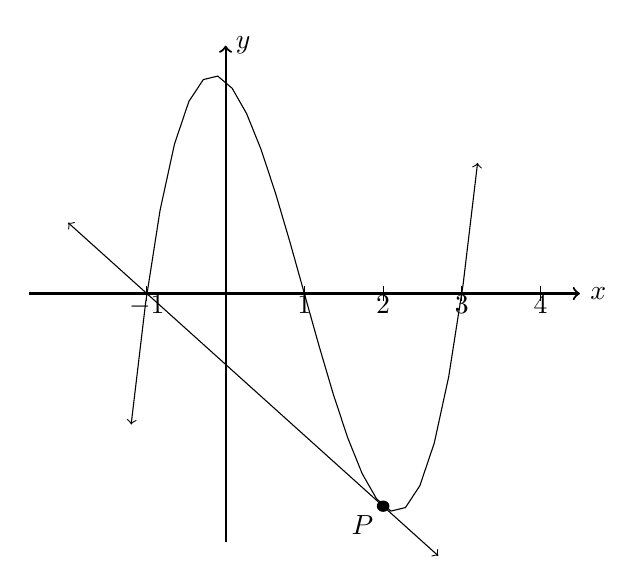
\begin{tikzpicture}[yscale=0.9]
        \foreach \x in {-1,1,2,3,4}
          \draw[shift={(\x,0)},color=black] (0pt,-3pt) -- (0pt,3pt) node[below]  {$\x$};
        %\foreach \y in {-5,-4,-3,-2,-1,1,2,3}
          %\draw[shift={(0,\y)},color=black] (2pt,0pt) -- (-2pt,0pt) node[left]  {$\y$};
          \draw [thick, ->] (-2.5,0) -- (+4.5,0) node [right] {$x$};
          \draw [thick, ->] (0,-3.5) -- (0,3.5) node [right] {$y$};
        %\fill (1,-4.5) circle[radius=2pt] node [below] {$P$};
        %\fill (0,-4) circle[radius=2pt] node [right] {$Q$};
        \draw [<->] plot[domain= -1.2:3.2] (\x, {(\x+1)*(\x-1)*(\x-3)});
        \draw [<->] plot[domain= -2:2.7] (\x, {-\x-1});
        \fill (2,-3) circle[radius=0.08cm] node[below left]{$P$};
    \end{tikzpicture}
    \end{center}
    A tangent to the function at $x=2$ is drawn with the point of tangency $P$.
    \begin{enumerate}%[itemsep=0.8cm]
      \item Find the coordinates of $P$. \hfill [1]
      \item Write down the derivative of the function, $f'(x)$. \hfill [2]
      \item Show that the gradient of the tangent line is $-1$. \hfill [1]
      \item Write down the equation of the tangent line. \hfill [2]
    \end{enumerate}
    \begin{tikzpicture}
      \draw (0,0) rectangle (15.2,9);
      \draw (8,0) rectangle (15.2,4.5);
      \node at (0,9)[below right]{\textbf{Working:}};
      \node at (8,4.5)[below right]{\textbf{Answers:}};
      \draw [dotted] (9,3.1)node[left]{(a)}--(15,3.1);
      \draw [dotted] (9,2)node[left]{(b)}--(15,2.0);
      \draw [dotted] (9,0.5)node[left]{(d)}--(15,0.5);
  \end{tikzpicture}

  \newpage
    \item Find the solutions for the system, the value(s) for $x$ such that $f(x)=g(x)$. Sketch the graph to show working.
    \begin{enumerate}
        \item $f(x)=-2x^2+3x+5$ \\[0.25cm] $g(x)=-2x+1$ \hfill [3] \vspace{0.3cm}
        % x=-0.367, 3.137
    \end{enumerate}
        \begin{tikzpicture}
            \draw (0,0) rectangle (15.2,8);
            \draw (8,0) rectangle (15.2,3);
            \node at (0,8)[below right]{\textbf{Working:}};
            \node at (8,3)[below right]{\textbf{Answers:}};
            \draw [dotted] (9,1.7)node[left]{(a)}--(15,1.7);
            %\draw [dotted] (9,1)node[left]{(b)}--(15,1);
        \end{tikzpicture}

    \item Perform a linear regression on the data in the table, finding $y=ax+b$. 
        \begin{center}
        \begin{tabular}{|l|c|c|c|c|c|c|}
            \hline
            $x$ & 53 & 54 & 56 & 60 & 61 & 65 \\ 
            \hline 
            $y$ & 11.5 & 11.6 & 12.0 & 12.2 & 12.5 & 12.3 \\ 
            \hline 
            \end{tabular}
        \end{center}
        \begin{enumerate}
            \item Write down the value of $a$, $b$. \hfill [3]%a=0.0756630, b=7.6156006
            \item Write down the correlation coefficient $r$. \hfill [1] %r=0.88080983
            \item Use your regression line to estimate $y$ for $x=58$. \hfill [2] %y=12.004056
        \end{enumerate}
        \begin{tikzpicture}
            \draw (0,0) rectangle (15.2,7);
            \draw (8,0) rectangle (15.2,4.5);
            \node at (0,7)[below right]{\textbf{Working:}};
            \node at (8,4.5)[below right]{\textbf{Answers:}};
            \draw [dotted] (9.4,3.1)node[left]{(a)(i)}--(15,3.1);
            \draw [dotted] (9.5,2.4)node[left]{(ii)}--(15,2.4);
            \draw [dotted] (9,1.7)node[left]{(b)}--(15,1.7);
            \draw [dotted] (9,1)node[left]{(c)}--(15,1);
        \end{tikzpicture}

        
                   
\end{enumerate}
\end{document}


\newpage
    \item Apply the law of cosines, $c^2=a^2+b^2-2ab \cos \theta$.
    \begin{enumerate}
        \item $a=12.3$, $b=14.7$, $\theta = 71^\circ$. Find the third side length, $c$. \hfill [3]
        \item $a=11.4$, $b=17.1$, $c=16.0$. Find $\hat{C}$ (the angle opposite side $c$). \hfill [3]
    \end{enumerate}
        \begin{tikzpicture}
            \draw (0,0) rectangle (15.2,5);
            \draw (8,0) rectangle (15.2,3);
            \node at (0,5)[below right]{\textbf{Working:}};
            \node at (8,3)[below right]{\textbf{Answers:}};
            \draw [dotted] (9,1.7)node[left]{(a)}--(15,1.7);
            \draw [dotted] (9,1)node[left]{(b)}--(15,1);
        \end{tikzpicture}


\item The data for $n=50$ are shown in the frequency table below.
    \begin{center}
        \begin{tabular}{|l|c|c|c|c|}
            \hline
            $x$ & $15 \leq x < 25$ & $25 \leq x < 35$ & $35 \leq x < 45$ & $45 \leq x < 55$\\ 
            \hline 
            Frequency & $k$ & 21 & 16 & 8\\ 
            \hline 
            \end{tabular}
    \end{center}
    \begin{enumerate}
        \item Find the value of $k$.  \hfill [1]
        \item Estimate the mean $\overline{x}$. \hfill [2]
        \item Estimate the standard deviation of the data, $\sigma$.  \hfill [2]
        \end{enumerate}
    \begin{tikzpicture}
        \draw (0,0) rectangle (15.2,5);
        \draw (8,0) rectangle (15.2,4);
        \node at (0,5)[below right]{\textbf{Working:}};
        \node at (8,4)[below right]{\textbf{Answers:}};
        \draw [dotted] (9,2.4)node[left]{(a)}--(15,2.4);
        \draw [dotted] (9,1.7)node[left]{(b)}--(15,1.7);
        \draw [dotted] (9,1)node[left]{(c)}--(15,1);
    \end{tikzpicture}
